% ============================
%          ABSTRACT/INTRODUCTION
% ============================

\chapter*{Introduction\markboth{Introduction}{}} 
\addcontentsline{toc}{chapter}{Introduction}
This thesis describes the development and applications of a laser turret with pan and tilt control: this device can be used to project a laser dot on a given surface (wall and/or floor) and finely control its position by solving the system’s inverse kinematics.

Once its functionality was validated, we used the turret for an human-robot interaction task.  In particular, we considered an existing system in which an operator interacts with a drone using pointing gestures \cite{gromov2018robot}; the system initially determines the relative localization between the two, then allows the operator to control the drone, which follows the indicated location in real time. The existing approach relied on a fast agile robot, and was unsuitable for implementation on slower or larger ground robots.  In this thesis, we demonstrate how the turret can be used with this goal. Figure \ref{fig:preview} gives an idea.
\begin{figure}
	\centering
	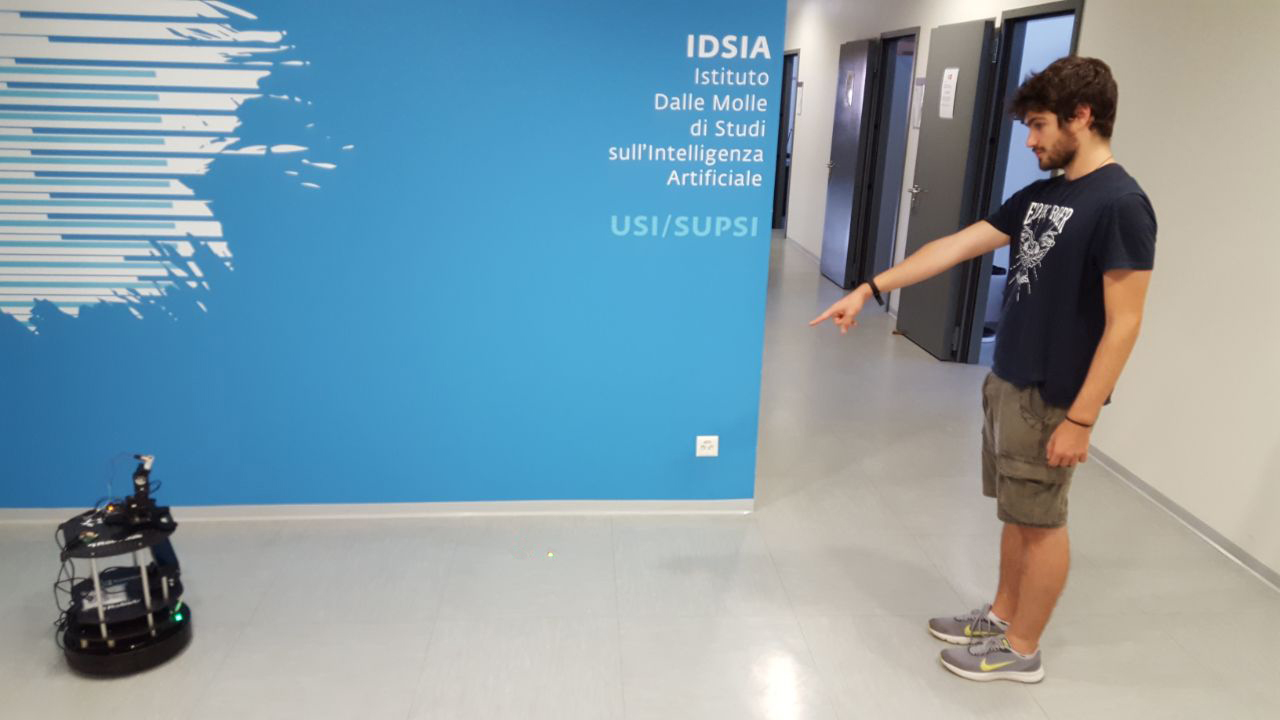
\includegraphics[width=\textwidth]{img/preview.jpg}%
	\caption{System Deployed to Drive a Ground Robot}
	\label{fig:preview}
\end{figure}

Finally, the turret was adopted to efficiently run experiments for fine tuning or validating different components of the system described above, such as the algorithms for relative localization and the algorithms for reconstruction of the pointed direction.  To this end, we ran an experimental campaign involving ten users.

\section*{Motivations and Related Works} \label{sec:related}
Many researches in the field of \ac{HRI} involve the study of interactions between an operator deployed alongside a robot in an environment they share. That means that a direct-line of sight exists between the two. Many interfaces have been proposed, ranging from standard joysticks (e.g. for low-level control of \acs{UAV}s) to hands-free gesture-based interfaces based on sensorized armbands~\cite{Wolf2013}, bracelets~\cite{Cacace2016,gromov2018video}, smartwatches~\cite{Villani2017} or voice commands~\cite{Gromov2016}.

The work developed in that thesis is collocated in that context, thus, an overview of related works is useful to understand motivations that stand behind that project.

\subsubsection*{Proximity HRI}
Proximity interaction techniques can take advantage of \emph{pointing gestures} to intuitively express locations or objects with minimal cognitive overhead; this modality has been often used in \ac{HRI} research e.g. for pick-and-place tasks~\cite{Brooks2006,Droeschel2011,Grossmann2014,Cosgun2015}, labeling and/or querying information about objects or locations~\cite{Brooks2006,Pateraki2014,Akkil2016}, selecting a robot within a group~\cite{Nagi2014a,Pourmehr2013}, and providing navigational goals~\cite{VanDenBergh2011,Abidi2013,Wolf2013,Jevtic2015,Gromov2016,Tolgyessy2017,gromov2018video}.

\subsubsection*{Pointing Based HRI Interface}
First, a differentiation can be made on sensing with respect to the type of sensors involved and their locations with respect to the human: it can be either \emph{external} or based on \emph{wearable} devices.
External sensing is usually based on vision systems, like regular \acs{RGB} cameras \cite{Pateraki2014,Monajjemi2016}, stereo cameras \cite{Nickel2003}, structured light depth cameras \cite{Cosgun2015} and \ac{ToF} cameras \cite{Droeschel2011}. The wearable sensing is typically realized either with inertial \cite{Wolf2013,Sugiyama2013} or magnetic measurements \cite{Bolt1980,Nickel2003}. 

Our work is an example of wearable sensing, as we exploit a wearable \ac{IMU} device. We are interested in such type of sensing because, even if vision-based methods are able to capture rich information about the objects, such as velocity, shape, size and color, they are susceptible to poor lighting conditions, low spatial resolution and may demand high computational resources.
Thus, for proximity interaction, wearable sensing is a very interesting possibility.

In particular, the use of pointing gestures constitutes a very practical and profitable solution, being based on mechanics which are natural for humans. This is why pointing gestures solutions are largely deployed to solve \ac{HRI} problems and significant research efforts have been devoted to this topic.
In fact, using pointing gestures as an input interface dates back to 1980s, when Bolt presented his now famous work ``Put-that-there''~\cite{Bolt1980}.
In the \ac{HRI} research, pointing gestures are often used for pick-and-place tasks~\cite{Brooks2006,Droeschel2011,Grossmann2014,Cosgun2015}, labeling and/or querying information about objects or locations~\cite{Brooks2006,Pateraki2014,Akkil2016}, selecting a robot within a group~\cite{Nagi2014a,Pourmehr2013}, and providing navigational goals~\cite{VanDenBergh2011,Abidi2013,Wolf2013,Jevtic2015,Gromov2016,Tolgyessy2017}.

Providing navigational goals is exactly the field in which our system finds one of its main applications and this is why we are now going to mention more works related to that task. First, however, it is worth to say that one important issue to be solved in natural human-robot interaction that involves pointing is a perception of the user's gestures. This can be a responsibility of a robot, i.e. the recipient of the message, as well as of a group of cooperatively-sensing robots~\cite{Giusti2012,Pourmehr2013}; of the environment~\cite{zivkovic2008toward}; or, as in our case, of a device worn by the user~\cite{Sugiyama2013,Wolf2013,Gromov2016}. The first approach is the most popular in \ac{HRI} research. However, it presents important challenges to solve the perception problem, and requires the robot to consistently monitor the user. Relying on sensors placed in the environment relaxes the requirements on the robots, but limits the applicability of the system to properly instrumented areas; in both cases, the positions being pointed at need to be inferred by external observation, which is typically performed with cameras or \acs{RGB-D} sensors.

\subsubsection*{Providing Navigational Goals}
Van Den Bergh et al. \cite{VanDenBergh2011} used pointed directions to help a ground robot to explore its environment. The robot continuously looks for a human in its vicinity and once detected begins the interaction. Using an \acs{RGB-D} sensor (Microsoft Kinect) the system detects human's hand and wrist. A vector connecting the center of the hand and the wrist is then projected on the ground, giving a principal exploration direction. Finally, the next exploration goal is automatically selected from a set of possible goals with respect to an instantaneous occupancy grid acquired by the robot. 

Similarly to the previous work, Abidi et al. \cite{Abidi2013} use a Kinect sensor to extract pointed directions. Navigation goals are continuously sent to the ground robot, which reactively plans its motion and thus allows the user to correct his input on the fly. The main drawback, however, is that the robot has to ``keep an eye'' on the user in order to reach the final target. To estimate pointed locations authors suggest two approaches: (1)~a vector originating from the elbow and passing the hand/finger, and (2)~a vector originating from the eyes and also passing the hand/finger.

Jevtic at al. \cite{Jevtic2015} experimentally compared several interaction modalities in the user study of 24 participants. A ground robot equipped with a Kinect and other sensors was used. The study compares three interaction modalities: \ac{DPI}, person following, and pointing control in area- and waypoint-guidance tasks. The DPI modality requires the user to push the robot by hands, the torques generated at motors are measured via electrical current and then are fed to a friction-compensation controller that drives the robot in the appropriate direction. The person following modality makes the robot to follow the user at a safe distance, the user can stop the robot at any time by raising her left hand above the left elbow and thus can control the robot's precise location. The pointing modality allows the user to command the robot's position with a pointing gesture, where the target location is calculated from the intersection of the ground plane with a line passing through the right elbow and the right hand of the user.
The authors measured task completion times, accuracy, and workload (with NASA-TLX questionnaire). Reported results show that the DPI modality is systematically better than the other modalities for all the metrics, while the pointing control shows the worst results.

Such a low performance of the pointing interface can be explained by a lack of appropriate feedback and a time-sparse nature of the implemented gesture control: the user issues a single command to drive the robot to a goal and see where the system ``thinks'' he was pointing at only when the robot reaches the target, therefore, the user is unable to efficiently correct the robot's position. This problem is nicely solved by our system, as it provides a real-time feedback to user pointing with a laser pointer, making him able to understand where the system thinks he is pointing and also correct any misalignment.

Problems reported in the study by Jevtic at al. \cite{Jevtic2015} are further aggravated by an inherently limited precision of a chosen pointing model (elbow-hand). As reported by many other works (see~\cite{Abidi2013,Nickel2007,Droeschel2011}), including those from the psychology research (see~\cite{Taylor1988,Herbort2016}), a more appropriate model would be a line that passes through the head and the fingertip. This is exactly the model we use for that thesis.

\subsubsection*{Wearable Sensors}
An alternative approach to a perception of pointing gestures is wearable sensors, as we mentioned before. 

Sugiyama et al. \cite{Sugiyama2013} developed a wearable visuo-inertial interface for on-site robot teaching that uses a combination of monocular camera and \ac{IMU} to capture hand gestures in the egocentric view of the user. The camera is also used for a monocular \ac{SLAM}, which allows to localize the user with respect to a common with the robot coordinate frame.

Wolf et al. \cite{Wolf2013} suggest a gesture-based interface for a robot control, that is based on a device they call BioSleeve, a wearable device placed on the user's forearm and comprised of a set of dry-contact surface \ac{EMGs} and an \ac{IMU}. Optionally, the authors suggest to strap an additional \ac{IMU} sensor on the upper arm to be able to perform a model-based arm pose reconstruction for pointing gestures. However, no information is given on how a user would localize herself with respect to the robot in order to control its position.

A work by Villan et al. \cite{Villani2017} suggests to use a single smartwatch device to control a drone. The system provides two interfaces: high-level commands and velocity commands.

Cacace et al. \cite{Cacace2016} demonstrate a multi-modal human-robot interface used for interaction in search and rescue missions. The operator is equipped with a Myo armband used for gestures, headset for voice commands, and a tablet with a touch screen.

\section*{Document Structure}
The rest of the document is structured in chapter as follows:
\begin{itemize}
    \item \textbf{Chapter 1 - Models Specification}  All the geometric models and formulas on which the system is based are explained. This includes turret model, human pointing model and relative localization procedure;
    \item \textbf{Chapter 2 - Hardware Implementation}  We introduce all the hardware components involved in the development of the presented system: servo motors and interface board for the turret, arm IMU devices and the ground robot used for demonstrations;
    \item \textbf{Chapter 3 - Software Implementation} We give an overview of the main libraries used and then describe the entire project software implementation;
    \item \textbf{Chapter 4 - Experiments and Applications} We describe the experiments the turret system allowed us to perform and show possible application scenarios developed;
    \item \textbf{Chapter 5 - Conclusion and Future Work} We make a brief recap of the thesis, draw some conclusions and report eventual further improvements or possible works;
    \item \textbf{Appendix A - Interesting Stuff} Here we collect a couple of things that did not find a place in the main document, but can be interesting to mention;
    \item \textbf{Appendix B - Code Listing} Relevant code listings.
\end{itemize}
